\section{Основные проблемы, влияющие на качество видеоконференций}

В современном мире на уровне сетевых коммуникаций возникают различные проблемы, влияющие на качество и надежность передачи данных, которые в конечном итоге могут негативно сказываться на качестве видеоконференций:
\begin{itemize}
	\item[--] Перегрузка сетей;
	\item[--] Потеря пакетов;
        \item[--] Пропускная способность сетей;
        \item[--] Jitter;
        \item[--] NAT;
        \item[--] MTU;
        \item[--] Reordering \cite{v4}.
\end{itemize}

Технология WebRTC представляет мощный набор инструментов, который способен решить эти проблемы, обеспечивая стабильное взаимодействие в реальном времени.

\subsection{Перегрузка сетей}

Одна из распространненых сетевых проблем -- перегрузка сетей, появляется, когда сетевой узел или линия связи переносит больше данных, чем может обрабатывать. Частые эффекты включают задержку в очереди, потерю пакетов или блокировку новых соединений, в худшем случае это может привести к снижению пропускной способности сети.

Для отслеживания и предотвращения перегрузки сетей существуют разные решения, например:
\begin{itemize}
	\item[--] Экспоненциальная выдержка -- это алгоритм, использующий обратную связь для мультипликативного уменьшения частоты некоторого процесса, чтобы постепенно, чтобы постепенно найти приемлимую частоту. Этот алгоритм обычно используется для планирования повторных отправок после коллизий. После первой коллизии каждый отправитель будет ждать 0 или 1 slot time. После второй коллизии отправители будут ждать где-то от 0 до 3 slot times включительно. По мере увеличения количества попыток повторной отправки число вариантов для задержки растет экспоненциально;
        \item[--] Приоритезация сетевых пакетов -- это метод, в котором пакеты, помеченные как "важные", пропускаются в первую очередь, а менее важные придерживаются, пока линия не освободится \cite{v11}.
\end{itemize}

\subsection{Потеря пакетов}

Потеря пакетов это частая проблема, которая характеризуется тем, что сообщения теряются при передаче, то есть не доходят до адресата. Для решения этой проблемы WebRTC предлагает несколько вариантов:
\begin{itemize}
	\item[--] Если были утеряны медиа-пакеты, то мы можем скрыть этот факт и восстановить пакеты самостоятельно, "догадываясь" о том, что было потеряно. Некоторые кодеки умеют восстанавливать потерянные кадры заменой их на тишину или путем повторения уже принятой речи, например, последнего кадра \cite{v8};
	\item[--] Retransmission (Ретрансляция) в случае, когда нас устраивают возникающие задержки, необходимые для запроса повторной отправки. Осуществляется RTP \cite{v9};
        \item[--] FEC (Forward Error Connection) -- это механизм, при котором медиапакета заранее дублируются и отправляются по сети несколько раз. Таким образом, даже если некоторые пакеты не будут получены, медиапоток все равно можно будет правильно разобрать и декодировать \cite{v10}.
\end{itemize}

\subsection{Пропускная способность сетей}

Начнем с определения пропускной способности сети -- это количество данных, которые можно передать по сети. Это динамическая величина, которая зависит от нагрузки, то есть от количества людей, использующих этот маршрут. Перегрузка сети в худшем случае может привести к потери пакетов, увеличению задержки и джиттера, что негативно сказывается на коммуникации в реальном времени.

Подход WebRTC заключается в том, чтобы попытаться оценить доступную пропускную способность сети и ограничить отправителя от отправки черезчур большего от нашей оценки. Оценка пропускной способности основана на эвристике, которая моделирует поведение сети и пытается его предугадать.

В WebRTC используются два основных подхода для оценки пропускной способности \cite{v5}:
\begin{itemize}
	\item[--] REMB \cite{v6};
	\item[--] transport-cc \cite{v7}.
\end{itemize}

\subsection{Jitter}

При отправке пакетов нет гарантии, что они будут доставлены в те же промежутки, с которыми были отправлены. Разница от ожидаемого интервала получения пакетов называется джиттером. Чем он выше, тем сильнее он влияет на качество передачи данных.

В виду того, что голос и видео чувствительны ко времени, при получении медиапакетов их необходимо собрать, переупорядочить и затем определять время, основываясь на последовательности и различиях, в которых они были сгенерированы, а не на последовательности и времени, в которых они были получены. Этим занимается буффер джиттера и в WebRTC имеется собственная реализация, которая учитывает задержку сети, любые наблюдаемые потери пакетов и "расстояние" между входящими аудио- и видеопакетами \cite{v12}.

\begin{figure}[ht]
\begin{center}
\scalebox{0.4}{
   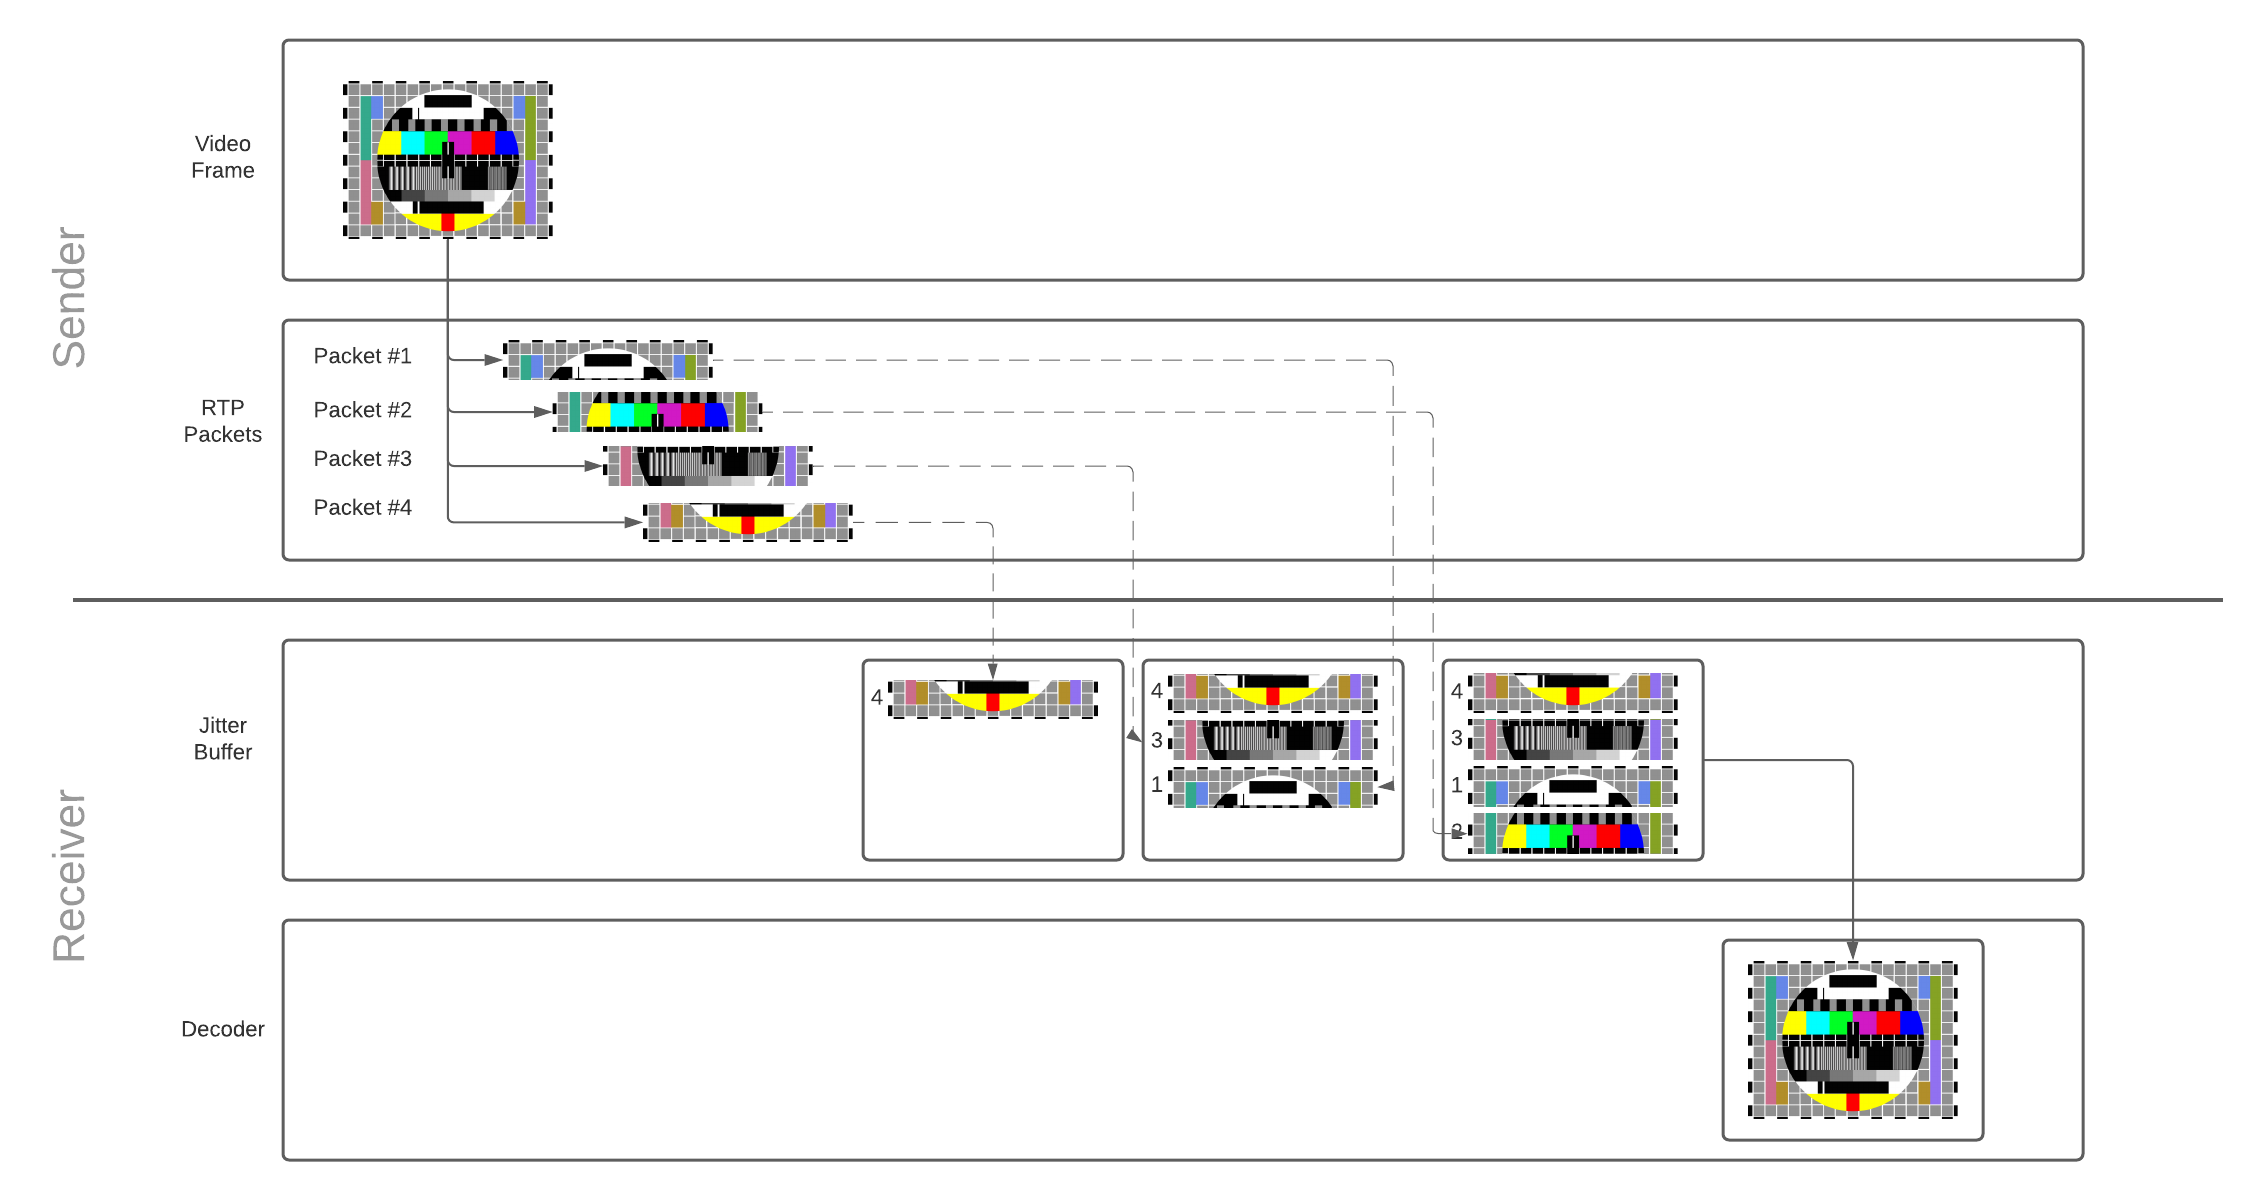
\includegraphics{images/jitter_buffer.png}
}

\caption{
\label{jitter-buffer}
     Джиттер буффер}
\end {center}
\end {figure}

Кратко алгоритм можно описать так, Рисунок ~\ref{jitter-buffer}:
\begin{itemize}
	\item[1.] Каждый пакет добавляется в буфер джиттера сразу после его получения;
	\item[2.] Как только пакетов становится достаточно для реконструкции кадра, пакеты, составляющие кадр, освобождаются из буфера и передаются для декодирования;
        \item[3.] Декодер, в свою очередь, декодирует и отрисовывает видеокадр на экране пользователя.
\end{itemize}

Поскольку буфер джиттера имеет ограниченную емкость, пакеты, которые остаются в буфере слишком долго, отбрасываются \cite{v13}.

\subsection{NAT}

NAT расшифровывается как трансляция сетевых адресов, обычно располагается между частной и публичной сетями и встроена в устройства сетевой маршрутизации. Входящий трафик в частную сеть направляется через привязку публичного адреса, которая возникает на устройстве NAT.

WebRTC должен иметь возможность передевать медиа между двумя абонентами, которые могут находиться за NAT устройствами, для этого необходимо, чтобы внешние пакеты могли проходить во внутреннюю сеть. STUN (Session Traversal Utilities for NAT) -- это стандартный метод обхода NAT, используемый в WebRTC \cite{v26}.

\begin{figure}[ht]
\begin{center}
\scalebox{0.5}{
   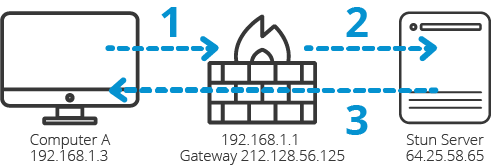
\includegraphics{images/stun.png}
}

\caption{
\label{stun}
     STUN}
\end {center}
\end {figure}


STUN-сервер позволяет своим клиентам находить публичный адрес, тип NAT, за которым они находятся и порт Интернета, связываемый NAT с конкретным локальным портом, Рисунок ~\ref{stun}. Затем эта информация используется WebRTC для настройки связи UDP между клиентами. Протокол STUN определяется стандартом RFC 3489 \cite{v25}.

\begin{figure}[ht]
\begin{center}
\scalebox{0.5}{
   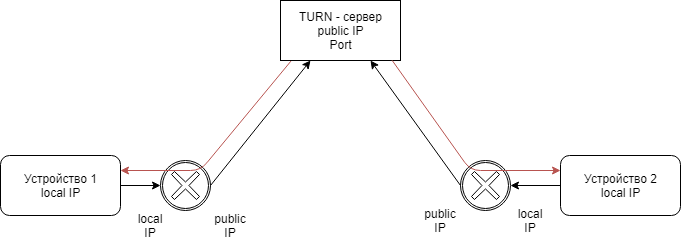
\includegraphics{images/turn.png}
}

\caption{
\label{turn}
     TURN}
\end {center}
\end {figure}

TURN (Traversal Using Relays around NAT) используется для передачи мультимедиа через сервер TURN, когда использование STUN невозможно. Решение о том, использовать STUN или TURN, принимается протоколом ICE. TURN-сервер фактически выступает проксирующим звеном между двумя клиентами, пропуская через себя весь трафик, Рисунок ~\ref{turn}.

ICE (Interactive Connection Establishment) -- это еще одно дополнение к протоколам STUN и TURN. Его задачи:
\begin{itemize}
	\item[--] Собрать данные об интерфейсах;
        \item[--] Проверить удаленные сервера STUN;
        \item[--] Проверить удаленные сервера TURN;
        \item[--] Проверить возможность установления соединения.
\end{itemize}

ICE выбирает самый легкий для прохождения маршрут (процедура номинирования пар) и выполняет проверку доступности между пиром и клиентом (могут ли они достучаться друг до друга). Приоритезация такая: без STUN сервера -- самый высокий приоритет, с использованием STUN -- пониже, с TURN -- самый низкий \cite{v27}.

\subsection{MTU}

MTU (Maximum Transmission Unit) -- это максимальный размер пакета, который может быть передан по сети. Если пакет передается с MTU большим, чем максимальный MTU на сети, то этот пакет фрагментируется. Конечно, он потом соберется обратно, однако если потеряется какая-то часть пакета, то потеряются все пакеты, поэтому необходимо оптимально работать с таким размером пакета, который соответствует MTU сети \cite{v4}.

WebRTC устанавливает размер MTU около 1200 байт и использует его для своих расчетов пакетирования (плюс-минус несколько байт). Использование такого значения гарантирует, что WebRTC будет хорошо работать в большинстве сетевых конфигураций \cite{v14}.

\subsection{Reordering}

Во время путешествия сетевых пакетов между источником и пунктом назначения есть вероятность переупорядочивания пакетов, то есть пакеты могут прибыть в другом порядке относительного того, в каком они были отправлены источником.

Для приложений видеоконференций, использующий протокол UDP и не использующих, например, метод коррекции ошибок вперед (FEC), переупорядочивание пакетов является проблемой, поскольку обычно приводит к потере данных, поскольку пакеты, приходящие не по порядку, отбрасываются, в худшем случае можно потерять целый видеокадр или аудиосегмент.

\begin{figure}[ht]
\begin{center}
\scalebox{0.6}{
   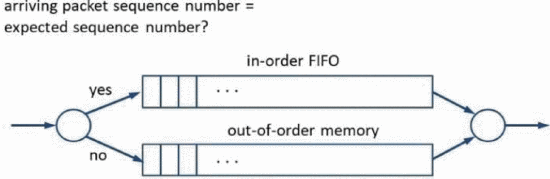
\includegraphics{images/out_of_order_memory.png}
}

\caption{
\label{out-of-order}
     Упорядочивающая архитектура с одной out-of-order памятью}
\end {center}
\end {figure}

Один из простейших методов коррекции переупорядочивания пакетов заключается в наличии памяти для неупорядоченных пакетов, в которой хранятся все пакеты, полученные с неожиданным порядковым номером. Эта память затем проверяется, когда ожидаемый номер не присутствует в конце очереди FIFO. Идея проиллюстрирована на Рисунке ~\ref{out-of-order}. Out-of-order буфер может быть организован как FIFO для простой коррекции переупорядочивания \cite{v15}.

\pagebreak